\documentclass[12pt,oneside,openright,a4paper]{cpe-english-project}

\usepackage{polyglossia}
\setdefaultlanguage{english}
\setotherlanguage{thai}
\newfontfamily\thaifont[Script=Thai,Scale=1.23]{TH Sarabun New}
\defaultfontfeatures{Mapping=tex-text,Scale=1.0,LetterSpace=0.0}
\setmainfont[Scale=1.0,LetterSpace=0,WordSpace=1.0,FakeStretch=1.0]{Times New Roman}
\emergencystretch=10pt
%\XeTeXlinebreaklocale "th_TH"	
%\XeTeXlinebreakskip = 0pt plus 1pt
%\setmathfont(Digits)[Scale=1.0,LetterSpace=0,FakeStretch=1.0]{Times New Roman}


%%%%%%%%%%%%%%%%%%%%%%%%%%%%%%%%%%%%%%%%%%%%%%%%%%%%%%%%%%%%%%%%%%%
% Customize below to suit your needs 
% The ones that are optional can be left blank. 
%%%%%%%%%%%%%%%%%%%%%%%%%%%%%%%%%%%%%%%%%%%%%%%%%%%%%%%%%%%%%%%%%%%
% First line of title
\def\disstitleone{DENTAL AI CHATBOT FOR DIAGNOSTICS AND POST-SURGERY CARE}   
% Your first name and lastname
\def\dissauthor{MR. CHANON KHANIJOH}   % 1st member
%%% Put other group member names here ..
\def\dissauthortwo{MR. PECHDANAI SAEPONG}   % 2nd member (optional)
\def\dissauthorthree{MS. FASAI SAE-TAE}   % 3rd member (optional)
\def\dissauthorID{63070503408}              % Author of dissertation
\def\dissauthortwoID{63070503434}              % Author of dissertation
\def\dissauthorthreeID{63070503436}   
\def\dissauthorEMAIL{chanon.kha@mail.kmutt.ac.th}              % Author of dissertation
\def\dissauthortwoEMAIL{pechdanai.sp@mail.kmutt.ac.th}              % Author of dissertation
\def\dissauthorthreeEMAIL{fasai.sae@mail.kmutt.ac.th}  


% The degree that you're persuing..
\def\dissdegree{Bachelor of Engineering} % Name of the degree
\def\dissdegreeabrev{B.Eng} % Abbreviation of the degree
\def\dissyear{2023}                   % Year of submission
\def\thaidissyear{2566}               % Year of submission (B.E.)

%%%%%%%%%%%%%%%%%%%%%%%%%%%%%%%%%%%%%%%%%%%%
% Your project and independent study committee..
%%%%%%%%%%%%%%%%%%%%%%%%%%%%%%%%%%%%%%%%%%%%
\def\dissadvisor{Dr. Unchalisa Taetragool , Ph.D.}  % Advisor
%%% Leave it empty if you have no Co-advisor
\def\disscoadvisor{Dr. Vorapat Trachoo, D.D.S., M.D.}  % Co-advisor
%%% Leave it empty if you have no Co-advisor 2
\def\disscoadvisortwo{Dr. Kritsasith Warin, D.D.S.}  % Co-advisor 2

\def\worktype{Project} %%  Project or Independent study
\def\disscredit{3}   %% 3 credits or 6 credits


\def\fieldofstudy{Computer Engineering} 
\def\department{Computer Engineering} 
\def\faculty{Engineering}
 
\def\appendixnames{Appendix} %%% Appendices or Appendix

% Change the line spacing here...
\linespread{1.15}

%%%%%%%%%%%%%%%%%%%%%%%%%%%%%%%%%%%%%%%%%%%%%%%%%%%%%%%%%%%%%%%%
% End of personal customization.  Do not modify from this part 
% to \begin{document} unless you know what you are doing...
%%%%%%%%%%%%%%%%%%%%%%%%%%%%%%%%%%%%%%%%%%%%%%%%%%%%%%%%%%%%%%%%


%%%%%%%%%%%% Dissertation style %%%%%%%%%%%
%\linespread{1.6} % Double-spaced  
%%\oddsidemargin    0.5in
%%\evensidemargin   0.5in
%%%%%%%%%%%%%%%%%%%%%%%%%%%%%%%%%%%%%%%%%%%
%\renewcommand{\subfigtopskip}{10pt}
%\renewcommand{\subfigbottomskip}{-5pt} 
%\renewcommand{\subfigcapskip}{-6pt} %vertical space between caption
%                                    %and figure.
%\renewcommand{\subfigcapmargin}{0pt}

\renewcommand{\topfraction}{0.85}
\renewcommand{\textfraction}{0.1}

\newtheorem{theorem}{Theorem}
\newtheorem{lemma}{Lemma}
\newtheorem{corollary}{Corollary}

\def\QED{\mbox{\rule[0pt]{1.5ex}{1.5ex}}}
\def\proof{\noindent\hspace{2em}{\itshape Proof: }}
\def\endproof{\hspace*{\fill}~\QED\par\endtrivlist\unskip}
%\newenvironment{proof}{{\sc Proof:}}{~\hfill \blacksquare}
%% The hyperref package redefines the \appendix. This one 
%% is from the dissertation.cls
%\def\appendix#1{\iffirstappendix \appendixcover \firstappendixfalse \fi \chapter{#1}}
%\renewcommand{\arraystretch}{0.8}
%%%%%%%%%%%%%%%%%%%%%%%%%%%%%%%%%%%%%%%%%%%%%%%%%%%%%%%%%%%%%%%%
%%%%%%%%%%%%%%%%%%%%%%%%%%%%%%%%%%%%%%%%%%%%%%%%%%%%%%%%%%%%%%%%


\begin{document}
\pdfstringdefDisableCommands{%
\let\MakeUppercase\relax
}
\begin{center}
  
\includegraphics[width=2.8cm]{Image/KMUTT_Logo.png}
\end{center}
\vspace*{-1cm}


\maketitlepage 
\makesignaturepage 

%%%%%%%%%%%%%%%%%%%%%%%%%%%%%%%%%%%%%%%%%%%%%%%%%%%%%%%%%%%%%
%%%%%%%%%%%%%%%% ToC, List of figures/tables %%%%%%%%%%%%%%%%
%%%%%%%%%%%%%%%%%%%%%%%%%%%%%%%%%%%%%%%%%%%%%%%%%%%%%%%%%%%%%
% The three commands below automatically generate the table 
% of content, list of tables and list of figures
\tableofcontents                    
\listoftables
\listoffigures                      

%%%%%%%%%%%%%%%%%%%%%%%%%%%%%%%%%%%%%%%%%%%%%%%%%%%%%%%%%%%%%%
%%%%%%%%%%%%%%%%%%%%% List of symbols page %%%%%%%%%%%%%%%%%%%
%%%%%%%%%%%%%%%%%%%%%%%%%%%%%%%%%%%%%%%%%%%%%%%%%%%%%%%%%%%%%%
% You have to add this manually..
\listofsymbols
\begin{flushleft}
\begin{tabular}{@{}p{0.07\textwidth}p{0.7\textwidth}p{0.1\textwidth}}
\textbf{SYMBOL}  & & \textbf{UNIT} \\[0.2cm]
$\alpha$ & Test variable\hfill & m$^2$ \\
$\lambda$ & Interarival rate\hfill &  jobs/second\\
$\mu$ & Service rate\hfill & jobs/second\\
\end{tabular}
\end{flushleft}
%%%%%%%%%%%%%%%%%%%%%%%%%%%%%%%%%%%%%%%%%%%%%%%%%%%%%%%%%%%%%%
%%%%%%%%%%%%%%%%%%%%% List of vocabs & terms %%%%%%%%%%%%%%%%%
%%%%%%%%%%%%%%%%%%%%%%%%%%%%%%%%%%%%%%%%%%%%%%%%%%%%%%%%%%%%%%
% You also have to add this manually..
\listofvocab
\begin{flushleft}
\begin{tabular}{@{}p{1in}@{=\extracolsep{0.5in}}p{0.73\textwidth}}
ABC & Adaptive Bandwidth Control \\
MANET & Mobile Ad Hoc Network  \\
Test & Lorem ipsum dolor sit amet, consectetur adipiscing elit. Nullam non condimentum purus. Pellentesque sed augue sapien. In volutpat quis diam laoreet suscipit. Curabitur fringilla sem nisi, at condimentum lectus consequat vitae.
\end{tabular}
\end{flushleft}

%\setlength{\parskip}{1.2mm}

%%%%%%%%%%%%%%%%%%%%%%%%%%%%%%%%%%%%%%%%%%%%%%%%%%%%%%%%%%%%%%%
%%%%%%%%%%%%%%%%%%%%%%%% Main body %%%%%%%%%%%%%%%%%%%%%%%%%%%%
%%%%%%%%%%%%%%%%%%%%%%%%%%%%%%%%%%%%%%%%%%%%%%%%%%%%%%%%%%%%%%%


\chapter{Introduction}
\section{Keywords}
\qquad Keywords: Oral Surgery, Dentistry, Diagnose, Follow-up, Artificial Intelligence, Chatbot, Machine Learning, Natural Language Processing

\section{Problem Statement}
  \subsection{Problem Statement and Motivation}
    \qquad Individuals seeking healthcare in today's world often run into a number of challenges while attempting to acquire correct information regarding their symptoms and appropriate treatment. Many patients have minor illnesses or symptoms that might not necessarily require immediate medical attention from a doctor. Nevertheless, these individuals usually resort to clinics or hospitals for a diagnosis as there is a lack of information and assistance available. \par
    \qquad This rise in patient visits not only places a considerable burden on healthcare facilities but also results in financial implications for patients themselves. The associated costs, such as consultation fees, diagnostic tests, and travel expenses, can impose an unreasonable financial strain on individuals. Moreover, this increased demand for medical attention has contributed to an imbalance in the doctor-to-patient ratio, affecting the overall quality of healthcare services provided. According to the National Statistical Office, the ratio of doctor-to-patient ratio is 1 to 8,057.\par
    \qquad Furthermore, the challenges do not cease once treatment is initiated. After receiving medical care, many patients still have many concerns about their health conditions. Many patients desire prompt answers to their worries about their conditions. In addition to these concerns, patients often have recurring questions, commonly categorized as frequently asked questions (FAQs).\par
    \qquad Regrettably, doctors and medical staff find themselves overwhelmed by the immense workload caused from the increased patient influx. As they aim to deliver quality care and diagnosis, they may have limited time and resources to respond satisfactorily to the patients.\par
    \qquad To address these pressing issues and enhance the healthcare experience for both patients and healthcare providers, we were motivated to develop an application that can effectively address these issues. The application will have the capability to diagnose common diseases and answer frequently asked questions from the patient's symptoms. Additionally, it will feature a chatbot designed to follow up on patient conditions after surgery.\par


  \subsection{Potential Benefits}
    \qquad The purpose of this dental application is to reduce frequently asked questions from patients regarding oral symptoms or diseases and also help with post-surgery follow-up thus reducing the workload of the dentist and medical staff. Dentists can use the extra time they gain to concentrate on patients who require more extensive care.\par
    \qquad In addition to the benefits that doctors receive from this application, patients and the general public also get their benefit as they have immediate access to oral diagnosis and knowledge. Since patients can understand their symptoms and get guidance on simple treatments, this helps to decrease needless doctor visits. Moreover, it can benefit patients by decreasing the expense of visiting the doctor to get a diagnosis. Another benefit that patients receive is continuous monitoring of their symptoms, which allows their doctor to be informed of any unexpected post-surgery problems.\par

\section{Objectives}
  \begin{itemize}
    \item To acquire the knowledge and skills necessary for developing an AI-powered chatbot. 
    \item To build a chatbot specialized in providing accurate answers to specific dental questions.
    \item To reduce doctors and staff by minimizing repeated questions and explanations from patients.
  \end{itemize}

\section{Expected Result}
  \qquad This project aims to develop a chatbot utilizing advanced natural language processing and machine learning techniques to be able to address frequently asked questions related to oral surgeries and be able to perform post-surgery follow-up. The chatbot is expected to provide an accurate response. \par  

\section{Scope of Work}
  \qquad The scope of this project involves the development of a chatbot designed to address frequently asked questions related to oral surgeries and provide post-surgery follow-up support. The chat bot will utilize natural language processing (NLP) and machine learning algorithms. The primary functions of the chatbot includes answering queries about each surgery, performing post-surgery follow-up, offering guidance and suggestions. Our primary focus will be on 4 specific surgical operations: Tooth Extraction, Wisdom Tooth Removal, Periodontal Surgery, Dental Implant Surgery. \par
  \qquad The final deliverable of this project will be a fully functional chatbot integrated into a web application, able to handle a range of frequently asked questions and perform post-surgery follow-ups. The project involves extensive research into relevant dentistry information, the development and training of machine learning models for question answering, and the design and implementation of the user interface. A usability test will be conducted to assess the effectiveness and user-friendliness of the chatbot and the associated web application. \par

\section{Project Schedule}
  \subsection{Semester 1}
    \begin{enumerate}
      \item Proposal
        \begin{itemize}
          \item Discuss Project with Advisors
          \item Kick-off meeting
          \item Write Project Idea
          \item Write Proposal Report
          \item Make Proposal Presentation          
        \end{itemize}
      \item Project Planning
        \begin{itemize}
          \item Collect Requirement
          \item Plan Task Schedule          
        \end{itemize}
      \item Learning and Research
        \begin{itemize}
          \item Research on Methodology
          \item Research On Oral Symptoms and FAG
          \item Research on Related Paper
          \item Study 4 Specific Oral Surgical Operations
          \item Study Post Surgery Follow-Up Procedure
        \end{itemize}
      \item Collect Data
        \begin{itemize}
          \item Prepare for Data Collecting
          \item Data Collecting
          \item Clean Data                 
        \end{itemize}
      \item Design and Data Preparation
        \begin{itemize}
          \item Make Use Case Diagram
          \item Make Architecture Diagram
          \item Design Ux/Ui
          \item Design AI Design
          \item Make Navigation Map                  
        \end{itemize}
      \item Implementation
        \begin{itemize}
          \item Select an Appropriate State-of-the-art AI Model
          \item Select an Appropriate Chatbot Framework 
          \item Select an Appropriate Front End Framework                 
        \end{itemize}
      \item Final Report
        \begin{itemize}
          \item Write Final Report
          \item Make Final Presentation              
        \end{itemize}
    \end{enumerate}

  \subsection*{Deliverables for Term 1}
    \begin{itemize}
      \item Final Proposal
      \item Use case diagram
      \item Architecture Diagram
      \item Navigation map
      \item ER Diagram
      \item Customer Journey
      \item Final UX/UI design
      \item Survey dental FAQ questionnaire for diagnosis and follow-up
    \end{itemize}
    \begin{figure}[!h]
      \centering
      \fbox{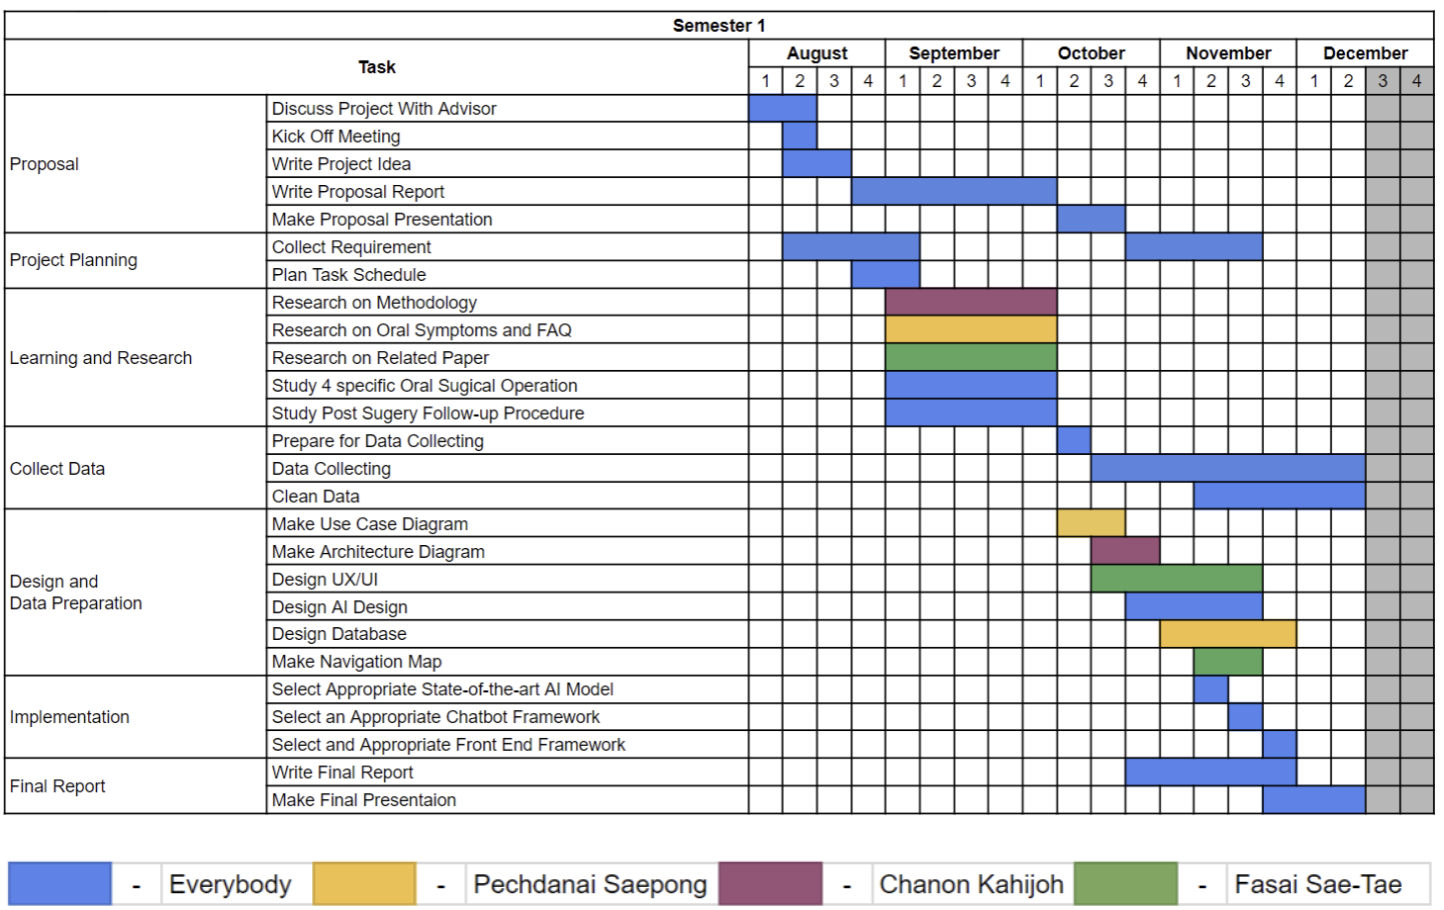
\includegraphics[width=.9\textwidth]{Image/Term1_Gantt.png}}
      \caption{Semester 1 plan schedule}\label{fig:Term1_Gantt}
    \end{figure}
    \begin{figure}[!h]
      \centering
      \fbox{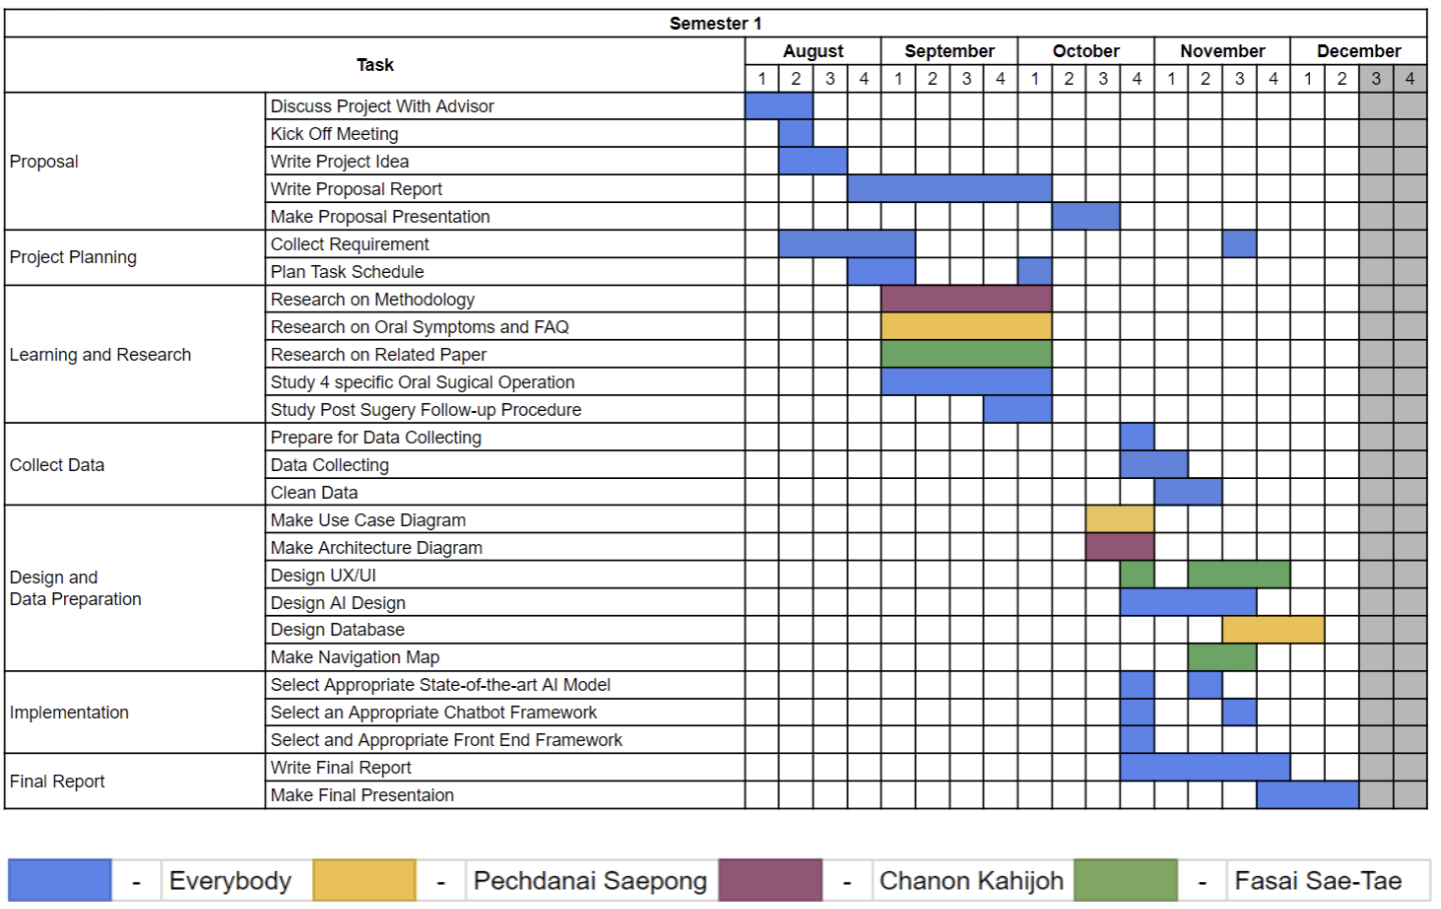
\includegraphics[width=.9\textwidth]{Image/Term1_Gantt_Actual.png}}
      \caption{Semester 1 actual schedule}\label{fig:Term1_Gantt_Actual}
    \end{figure}

  \subsection{Semester 2}
    \begin{enumerate}
      \item Deep Learning and Chatbot Implementation
        \begin{itemize}
          \item Model Implement
          \item Model Training
          \item Model Testing and Evaluation
        \end{itemize}
      \item Web Application Implementation
        \begin{itemize}
          \item Backend
          \item Frontend
          \item Test Case Design
          \item Unit Testing
          \item Usability Testing
        \end{itemize}
      \item Semester 2 Report
        \begin{itemize}
          \item Write Semester Report
          \item Semester Presentation
        \end{itemize}
    \end{enumerate}

  \subsection*{Deliverables for Term 2}
    \begin{itemize}
      \item Mobile application in both iOS and Android platform
      \item Testing result
      \item Feedbacks from users
      \item Senior Project Report
    \end{itemize}
    \begin{figure}[!h]
      \centering
      \fbox{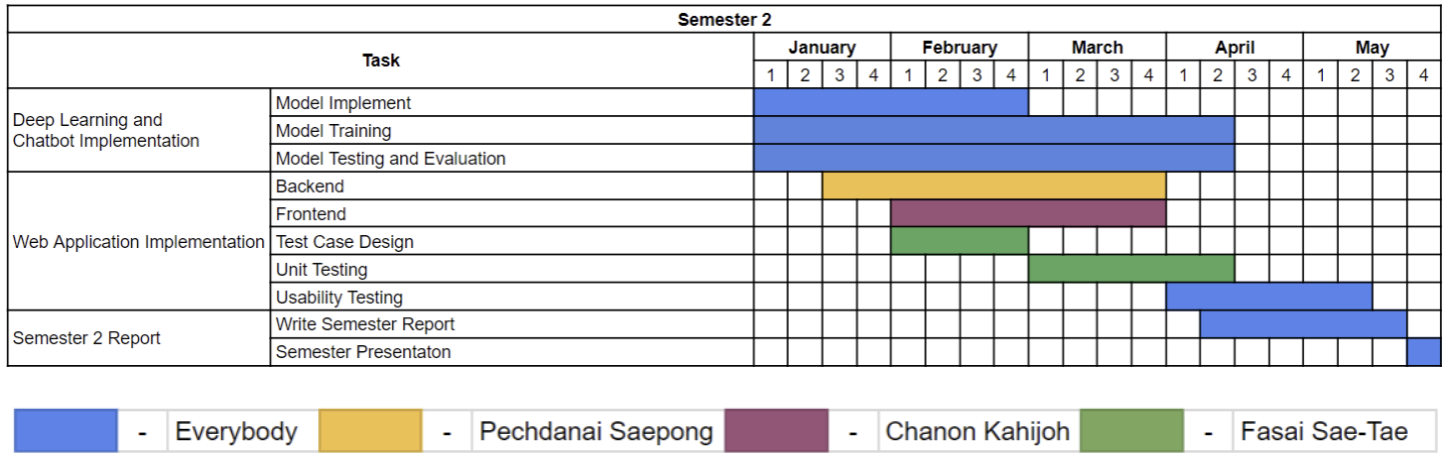
\includegraphics[width=.9\textwidth]{Image/Term2_Gantt.png}}
      \caption{Semester 2 plan schedule}\label{fig:Term2_Gantt}
    \end{figure}

\chapter{THEORY AND RELATED RESEARCH}
\section{Introduction}
  \qquad This chapter will explain the details of the core concept and the solution planning. Theory and core concepts, languages and technologies, and related research will be discussed in this chapter. First, we will cover the theory and core concept of both dentistry and artificial intelligence. Second, programming languages and technologies that are intended to be used in this project will be described in the “Languages and Technologies” section. Lastly, related research and similar solution approaches to the objective will be discussed in the “Related Research and Competing Solutions” section.

\section{Theory and Core Concepts}
  \qquad Common oral problems, including tooth decay, wisdom teeth complications, and gum disease, require consistent treatment for a considerable number of patients. Dentists, who routinely engage with patient inquiries and symptom tracking, have recommended that our focus be directed towards Tooth Extraction, Wisdom Tooth Removal, Periodontal Surgery, and Dental Implant Surgery. These specific procedures directly address the aforementioned common oral problems, aligning our work with the suggestions of dental professionals.\par
  \subsection{Tooth Extraction}
    \qquad Tooth extraction is a common dental procedure performed by a dentist or oral surgeon to remove a tooth from its socket in the jawbone. It is necessary for various reasons, including extensive tooth decay, crowding, tooth impaction, or as part of orthodontic treatment. Recovery typically takes a few days to a few weeks. The benefits of tooth extraction vary depending on the reason for the procedure. However, the disadvantages of tooth extraction often include challenges with chewing food and a potential loss of aesthetic appeal. Additionally, there may be complications that require careful monitoring, such as post-surgical swelling or infection.\par
  \subsection{Wisdom Tooth Removal}
    \qquad Wisdom tooth extraction, also known as third molar extraction, is a dental procedure performed to remove the third molars, commonly referred to as wisdom teeth. These teeth often become impacted or lead to various dental issues due to their slow growth and limited space in the jaw. Surgery becomes necessary for various reasons, including the prevention of pain arising from the inability of third molars to erupt properly or the prevention of issues related to crowded and misaligned teeth. However, the most common concerns associated with this procedure are the potential side effects after surgery, such as swelling, unusually significant or continuous discharge, or facial distortion lasting more than two weeks.\par

  \subsection{Periodontal Surgery}
    \qquad Periodontal surgery, also known as gum surgery, is a dental procedure aimed at treating various gum diseases and conditions. It involves the removal of infected gum tissue and, in some cases, the reshaping of the underlying bone to restore gum health and improve the stability of teeth. During this surgery, the dentist or periodontist carefully removes the diseased tissue and then shapes and contours the remaining gum and bone to promote optimal healing. In more advanced cases, bone grafts or tissue-stimulating proteins may be used to encourage tissue regeneration. Periodontal surgery is crucial in preventing the progression of gum diseases, reducing gum pockets, and ultimately preserving the natural teeth. Besides its significant impact on oral health, undergoing periodontal surgery can also enhance an individual's confidence and self-esteem by restoring a healthy, aesthetically pleasing smile.\par

  \subsection{Dental Implant Surgery}
    \qquad A dental implant is a technology used to replace missing teeth by employing sturdy materials as dental implants to serve as replacements for natural tooth roots. Presently, it is common to use dental implants that encompass both the root and the tooth, as they closely resemble natural teeth in appearance and function realistically. Additionally, they aid in preventing the deterioration of the jawbone where the implant is placed. To be a suitable candidate for dental implants, a patient must possess healthy gums and adequate bone support for the tooth roots. Following a root canal procedure, it is imperative for the patient to consistently maintain their oral health. Dental implants offer numerous advantages, including the prevention of teeth from shifting or becoming misaligned due to tooth loss, as well as contributing to the strengthening and preservation of oral hygiene.\par

\section{Languages and Technologies}
  \subsection{Web Development Language}
    \subsubsection{JavaScript}
      \qquad JavaScript, abbreviated as JS and developed by Netscape in the mid-1990s, is one of the most used programming languages in web development. It enables the development of dynamic content within web pages, enhancing websites responsiveness to user interactions.\par
      \qquad Operating as a scripting language on the client side, JavaScript runs directly within web browsers, facilitating interaction with the Document Object Model (DOM), which represents a webpage's structure and content.\par
      \qquad JavaScript boasts a rich set of features and capabilities, including support for various data types, loops, functions, and more. Moreover, it offers many libraries and frameworks that simplify complex tasks.\par
      \qquad A key attribute of JavaScript is its capacity to handle asynchronous operations. Asynchronous operations enable data retrieval without disrupting the user’s experience, as these operations occur independently through mechanisms such as async/await and Promises.\par
    \subsubsection{TypeScript}
      \qquad Developed by Microsoft, TypeScript (or TS) is an enhanced version of JavaScript, adding strong typing and advanced features to the original language.\par
      \qquad One of the most noticeable changes from default JavaScript is the introduction of a strong tying system. TypeScript requires variables, function parameters, and function return types to be explicitly defined with data types. This enhances error detection during the development process, resulting in fewer bugs when the website is deployed. It also promotes easier cooperation between developers, as the code becomes more understandable.\par
      \qquad TypeScript offers additional features, such as interfaces and custom type definitions, which enable objects to have specific shapes. This feature enhances code comprehension and facilitates integration with third-party libraries.\par
    
    \subsubsection{Python}
      \qquad Python, famous for its ease of use and readability, has gained in popularity in web programming due to its flexibility and an extensive collection of frameworks designed for web application development. It is frequently employed in web backend development, offering developers a wide range of frameworks and libraries to choose from. This diversity makes it an attractive choice for creating robust and scalable websites.\par

    \subsubsection{Hypertext Markup Language}
      \qquad Hypertext Markup Language, abbreviated as HTML, serves as the standard language for creating the structural framework of websites. It uses a markup syntax consisting of tags to define various components, including headings, paragraphs, links, images, etc. HTML’s simplicity, adaptability, and compatibility with multimedia features have solidified its enduring importance in the realm of website development. It stands as an indispensable tool for developing everything from straightforward web pages to complex websites.\par

    \subsubsection{Cascading Style Sheet}
      \qquad Cascading Style Sheets, abbreviated as CSS, is commonly referred to as a "style sheet." It is a language used to format HTML documents, with CSS being responsible for defining rules that specify the presentation of content within a document. These rules encompass aspects such as text color, background color, font type, and text positioning. The fundamental concept behind CSS is the separation of HTML document content from the instruction used for formatting its display. By employing this separation, CSS achieves two primary objectives. Firstly, it ensures that the document's display format is independent of its content, facilitating the task of formatting HTML documents, especially when the content undergoes frequent changes. Secondly, CSS enables precise control over the presentation format of HTML documents, ensuring consistency across all pages within the same website. Styling rules for HTML documents were initially introduced in HTML 4.0 back in 1996, in the form of CSS Level 1 recommendations established by the World Wide Web Consortium (W3C).\par

  
  \subsection{Front-end Framework}
    \qquad Front-end frameworks play a crucial role in web development by simplifying the creation of user interfaces. They encompass design, layout, and interactive elements such as forms and buttons. These frameworks provide pre-written code that includes HTML, CSS, and JavaScript components, facilitating code reuse and maintaining consistency across web projects. By leveraging front-end frameworks, developers can efficiently generate HTML and CSS, design responsive layouts for various devices, ensure a consistent user experience, automate repetitive tasks, and manage their code efficiently. Ultimately, front-end frameworks streamline and structure the development process, enabling the creation of user-friendly and visually appealing web applications. Examples of front-end frameworks are as follows:\par
    \begin{itemize}
      \item React: A front-end framework, React stands apart because of its virtual Document Object Model (DOM), which enhances its functionality. It is a perfect framework for those who expect high traffic and require a steady platform to manage it. 
      \item Angular: Formally released in 2016, the Angular framework was established by Google to bridge the gap between the mounting demands of technology and conventional notions that displayed the results. In contrast to React, Angular is distinctive with its two-way data binding trait. It means that there is real-time synchronization between the view and model, where any alteration in the model replicates promptly on the view and vice versa.To reduce doctors and staff by minimizing repeated questions and explanations from patients.
      \item Vue.js: It has a small size and offers two main benefits – a visual DOM and a component-based structure. It also employs two-way data binding. This front-end framework is versatile and assists with various tasks when building web applications. The difference between Vue and React is that Vue is a JS framework while React is a JS library. So, Vue is more suitable for large projects.
      \item Semantic-UI: The objective of Semantic lies in empowering the designers and developers by creating a language for sharing UI. It uses natural language that makes the entire code self-explanatory. The framework is comparatively new to the ecosystem. Still, with its striking user interface, simple functionalities, and features, it has become one of the most popular front-end frameworks.
      \item Next.js: Used by some of the world's largest companies, Next.js enables you to create full-stack web applications by extending the latest React features and integrating powerful Rust-based JavaScript tooling for the fastest builds.
    \end{itemize}

  \subsection{Backend Framework}
    \qquad A backend framework serves as a foundational platform for developers to expedite the creation of web and mobile applications with standardization. In the context of backend frameworks, they simplify server-side development by offering tools, libraries, and components that streamline the construction of web applications. These frameworks automate various aspects of web development, enhancing efficiency and cleanliness in code design. Examples of backend frameworks are as follows:\par
    \begin{itemize}
      \item ExpressJS: It is a minimal Node.js framework used to develop highly flexible applications.
      \item Django: Django is the most popular Python framework used in web development. Based on the Don’t Repeat Yourself (DRY) principle, Django focuses on code reusing, thus enhancing the development speed. It is also a very secure framework.
      \item Node.js: JavaScript is the most popular programming language in the world. With the emergence of Node.js, JavaScript’s popularity in the backend development community increased rapidly, and in the last decade, Node.js has become one of the top names.
      \item Flask: It’s a simple, highly flexible, and performing web framework. Being a lightweight framework, or micro-framework, it is easy to learn and understand Flask. Moreover, being a Python framework, it is very user-friendly.
    \end{itemize}
  
  \subsection{Chatbot}
    \qquad A chatbot is a machine learning (ML) or artificial intelligence (AI) system designed to simulate and handle human conversations, whether written or spoken. These AIs enable users to interact with digital devices as if they were having a conversation with a human. Chatbots can vary widely in complexity, from basic systems that respond to user queries to advanced digital assistants that learn and adapt over time, providing personalized experiences as they collect and process data.\par
    \subsubsection{Chatbot Framework}
      \qquad A Bot Framework is a platform where developers create and define the behavior of chatbots. It simplifies the complex task of building chatbots that can operate on various messaging platforms and software development kits (SDKs). While some frameworks claim “write once, deploy anywhere" capabilities, in practice, developers often need to create separate chatbots for each messaging platform. The Bot Framework comprises components such as the Bot Builder SDK, Bot Connector, Developer Portal, Bot Directory, and an emulator for testing. However, it may not be the best choice for beginners looking to learn chatbot development due to its complexity.\par
      \qquad Examples of Bot frameworks include:\par
      \begin{itemize}
        \item DialogFlow
        \item Microsoft Bot Framework
        \item Rasa
        \item Amazon Lex
        \item IBM Watson Assistant
        \item Wit.ai
        \item Botpress
      \end{itemize}
    
    \subsubsection{ Pretrained Chatbot Model}
      \qquad A pretrained chatbot model is a Natural Language Processing (NLP) model that has been trained on a wide range of text data from sources such as books, articles, social media, etc. These models are equipped with the capability to understand and generate text that closely resembles human language, making them valuable for chatbot development and other natural language tasks. These chatbots can also undergo fine-tuning or additional training for a specific task or domain to enhance their accuracy and performance.\par
      \paragraph{DeBERTa}\mbox{}\\
        \null\qquad DeBERTa (Decoding-enhanced BERT with disentangled attention) is a neural language model architecture designed to enhance the performance of pre-trained models like BERT (Bidirectional Encoder Representations from Transformers) and RoBERTa (Robustly optimized BERT approach) with two techniques, a disentangled attention mechanism and an enhanced mask decoder.\par
  


\chapter{EXPERIMENTAL RESULTS}

\end{document}
